%% ------------------------------------------------------------------------- %%
\chapter{Final Conclusions}
\label{cap:conclusoes}

\section{BEM Efficiency as a Computational Tool}

We can discuss the efficiency of BEM as a computational tool from the obtained results. 
The heavly parallel nature of BEM implies that we can allocate more computational resources 
to solve a problem which this method can be deployed as the number of meshes increases.

Since the GeForce GTX 980 provided good resuts in \texttt{Venus}, one can use a home 
computer paired with such videocard to execute the simulation in a reduced amout of time 
without investing into a powerful machine with, for example, two CPUs. Such GPUs can also 
be used to upgrade exisiting servers for even better speedups.

When compared to the original program, the total time elapsed in the simulation was reduced 
to a margin that is feasible for bigger mesh numbers such as the 14400 sample, as shown in 
Figure $\ref{fig:total_brucutuiv}$. It is important to mention that it is possible to archive even more speedups if a 
load balancer is implemented in a way that it can use both CPU and GPU in parallel.

If there is a major concern about errors in the simulation, perhaps caution is required when 
offloading the task to the GPU, as the mainly graphic on Figure $\ref{fig:ghmatecd_brucutuiv_error}$ 
indicates.

\begin{figure}[ht]
\centering
\textbf{Total elapsed time in \texttt{BrucutuIV}}\par\medskip
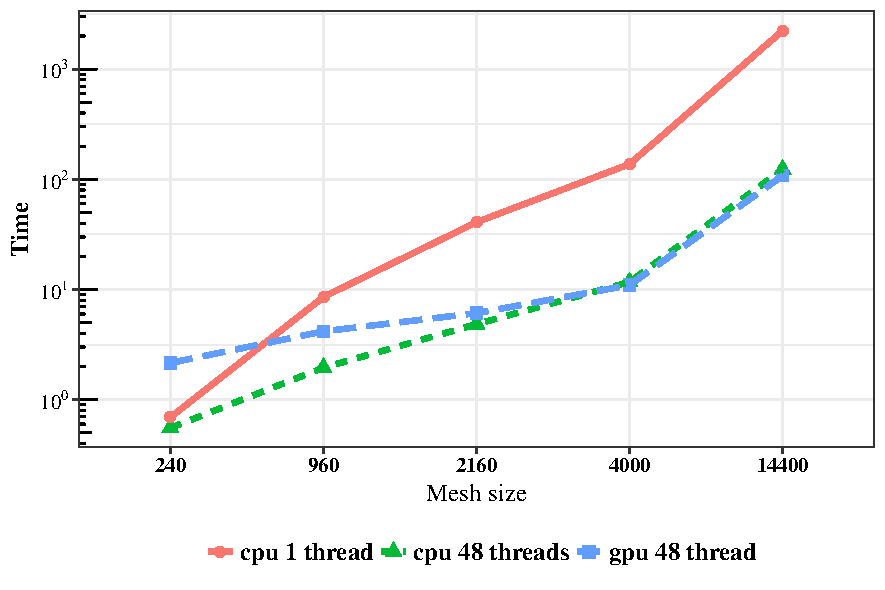
\includegraphics[scale=1]{total_brucutuiv.pdf}
\caption{Total elapsed time in \texttt{BrucutuIV}. One data per sample}
\label{fig:total_brucutuiv}
\end{figure}

As a final conclusion, the program can now be used to simulate cases where the original couldn't 
because of time constraints or unecessary memory usage.

\section{As a Programmer}

Adding features related to a technology that did not exist in the time period of the program's 
development was a challenge at first mainly because of sparse support for the original language nowdays. 
Sure, calling C from Fortran in the way we presented enabled the possibility of the current solution, 
but what if it couldn't be done in that way? That could be the case for even older systems.

Also, implementing numeric algorithms is no easy task because minor mistakes can cause an absurd change 
in the results, but without crashing the original program. Detecting what variable is the cause of the 
error is aways a toil. The use of automated tests to conclude what routine caused the error was determinant 
since the result of a routine is used as input for another, causing the origin of all problems to be lost. 
Even then, GDB proved to be a nice friend for detecting such problems. Tests are important and must 
not be underestimated.

As for the GPU development, testing the implementation of the algorithm there was extra painful as the developer 
can not run \texttt{X11} and \texttt{cuda-gdb} in the same GPU for testing. Additionaly, sometimes, 
a \texttt{SEGFAULT} in a CUDA kernel caused the computer to hang, needing a complete reboot of the machine. 
One last complain is that it is not possible to allocate multiple arrays in CUDA's shared memory dynamically, 
requiring pointer magic to allocate multiple arrays into a single array. These points require improvements 


